\cleardoublepage
\begin{TranslationNoMiniToc}
% 03_Translate.tex 开头
\counterwithout{figure}{subsection} % 取消图片序号与 section 的关联，使其全局连续
% 03_Translate.tex 开头

\section{外文翻译}

{\centering\zihao{3}\bfseries 通过分类确定性多普勒信号实现智能设备的手势识别\par}
\vspace{6pt}

\renewcommand{\theequation}{\arabic{equation}}
\renewcommand{\thefigure}{\arabic{figure}}

\subsection{摘要}
智能手机和平板电脑等个人设备正迅速成为个人通
信、信息和控制中心。除了多点触控屏幕之外，人类手势被视为
一种新型的人与智能设备交互界面。在本研究中，我们提出了一
种非接触式解决方案，用于在智能设备上实现手势识别。该方案
基于连续波、时分复用（$TDM$）、单输入多输出（$SIMO$）的
多普勒雷达传感器，可通过对现有智能设备射频前端进行轻微修
改来实现；同时结合机器学习算法，通过对确定性多普勒信号进
行分类来识别预定义的手势。我们搭建了一个模拟基于智能手机
雷达传感器的实验平台，实验结果验证了所提方法的鲁棒性和准
确性。关键词——分类，多普勒效应，手势识别（$HGR$），机
器学习，雷达架构。

\subsection{引言}
近年来，智能手机和平板电脑等个人设备已成为人类日常生活中不可或缺的工具。这些智能设备集成了无线接口、传感器和强大的计算能力，正迅速成为个人通信、信息和控制中心 $[1]$。迄今为止，人与智能设备之间的大多数交互仍基于多点触控屏幕 $[2]$。随着智能设备的应用扩展到虚拟现实以及电视（$TV$）和投影仪的无线控制等场景，基于人体手势识别（$HGR$）的非接触式交互吸引了越来越多的关注 $[3]$–$[6]$。

最初，非接触式手部手势识别（$HGR$）在计算机科学领域被视为一种人机界面（$HMI$） $[7]$。基于摄像头和数字图像处理算法，这种无线 $HMI$ 可归类为光学方法。由于高度依赖计算资源、直接视线以及照明条件，基于计算机视觉的 $HGR$ 应用至今仍受限 $[8]$。为了克服上述成本、障碍物和光照问题，研究人员已开始探索基于微波和毫米波的方法，即脉冲和连续波（$CW$）雷达方法的 $HGR$ $[9]$–$[18]$。

迄今为止，大多数已报道的基于 $HGR$ 均采用调频连续波（$FMCW$）方案 $[12]$-$[15]$, $[19]$, $[20]$。其中最著名的是 "$Google \ Soli$" $[15]$, 它是一个 $60 \ GHz$ 的 $FMCW$ 雷达模块，带宽高达 $7 \ GHz$。通过分类距离-多普勒频谱图 $[10]$, 它可以识别细微的手势，例如手指摩擦动作，可用于控制智能手机的音量或音乐播放列表等功能。然而，额外增加的毫米波雷达芯片及其外围组件会提高成本，增加功耗，并占用更多内部空间，而这些资源对于空间和资源受限的设备来说十分稀缺。

到目前为止，在上述基于雷达的解决方案中已提出了两类识别算法。其中一类基于线性方法，试图从后向散射场 $[4]$-$[6]$, $[9]$ 中提取目标的位移信息，即手势的运动模式。这类方法的优点是所提取的手势模式具有明确意义，能与实际手势直接对应。缺点是由于手部的米氏散射 $[21]$，检测到的模式形状会因照明角度不同而产生显著变化，从而增加了识别难度。

另一类算法基于人工智能（$AI$），利用人工神经网络（$ANN$）和基于机器学习的分类方法的非线性泛化能力 $[22]$-$[24]$。这些方法用于识别手势散射场的 "特征签名"。其优点在于，只要使用这些签名来训练基于 $ANN$ 的分类器 $[10]$, $[12]$-$[14]$, $[16]$, $[17]$, $[19]$, $[25]$, 就可以对任意预定义的手势实现 "黑箱式" 识别。对于此类黑箱分类，需要大量来自不同人员完成的手势数据以训练分类器。然而，所需训练手势的数量可能高达数万，导致在手势数据集采集、数据标注和数据清洗方面耗费大量人力和时间。

在本研究中，我们结合了上述架构和算法的优点，提出了一种在智能设备上实现手部手势识别（$HGR$）的系统性解决方案。该方案基于连续波（$CW$）、时分复用（$TDM$）、单输入多输出（$SIMO$）的多普勒雷达传感器（$DRS$）以及一种通过分类确定性多普勒信号来识别手势的机器学习算法。这种 $DRS$ 只需对现有智能设备的射频前端进行轻微修改即可实现，硬件成本、功耗和空间占用的增加可忽略不计。与 "黑盒" 分类不同，此类确定性多普勒信号具有明确的物理和数学意义，因此仅需使用单人完成的少量手势即可训练出分类器，并基于此获得对不同用户均具有高精度的手势识别能力。基于模拟智能手机 $DRS$ 系统的实验验证了所提出 $HGR$ 方法的鲁棒性和准确性。

本文其余部分组织如下。在第二部分中，回顾了相关现有的 $DRS$ 研究工作，并在此基础上介绍了基于智能手机的 $TDM \ SIMO \ DRS$ 架构以及专用于该 $DRS$ 的算法 。在第三部分中，推导了所提出 $DRS$ 的手势设计及相应算法。第四和第五部分分别提供了全波仿真和实验验证。最后，第六部分给出了结论。

\subsection{架构}
\subsubsection{架构}
\begin{figure}[htbp]
    \centering
    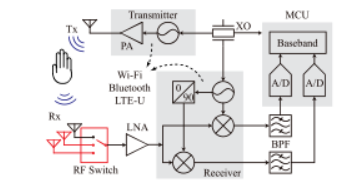
\includegraphics[width=0.75\linewidth]{assets/figs/image4.png}
    \caption{通过重构Wi\text{-} Fi和LTE\text{-}  URF信道实现TDM\text{-} SIMO\ DRS。红色绘制的设备为新增设备。}
    \label{fig:placeholder}
\end{figure}

随着射频集成电路（$RFIC$）的快速发展，在过去十年中已开发出小型化的连续波 $DRS$, 用于非接触式运动检测。目标运动包括人体生命体征 $[26]$-$[30]$ 和机械运动 $[31]$-$[33]$。最初使用的是单输入单输出（$SISO$）架构的连续波 $DRS$ $[26]$, $[27]$, $[29]$, $[30]$。在能够消除相位模糊的算法辅助下，可实现对一维运动的线性检测。对于二维运动，也实现了具有一路发射和两路接收通道的 $SIMO \ DRS$ $[4]$, $[36]$, $[37]$。然而，在上述所有 $SIMO \ DRS$ 中，发射和接收天线被布置在一条直线上，因此无法用于检测三维手势。此外，由于包含多个射频通道，它们也难以集成到智能设备中。

在本研究中，利用连续波差分接收信号（$CW \ DRS$）的超窄带特性，我们提出了一种时分复用-单发多收（$TDM$-$SIMO$）$DRS$, 该方案只需对传统智能设备中的现有射频前端进行轻微修改即可实现。其示意图如图1所示。

迄今为止，智能设备尤其是智能手机和平板电脑已经集成了多种无线接口。除了用于 $2G$、$3G$、$4G$ 和 $5G$ 通信的射频前端外，还有工作在 $2.4 \ GHz$ 和 $5.8 \ GHz$ 频段的 $Wi$-$Fi$、蓝牙以及长期演进（$LTE$）$-U \ [38]$ 信道。在大多数设备中，所有这些信道均采用共享同一参考振荡器和基带单元的标准数字中频架构实现。因此，这些信道可灵活选择用于实现适用于 $HGR$ 的 $2.4 \ GHz$ 或 $5.8 \ GHz$ 前端。

例如，可以将 $2.4 \ GHz$ 蓝牙的发射信道与 $2.4 \ GHz \ Wi$-$Fi$ 的接收信道结合，从而构成一个 $2.4 \ GHz$ 前端。类似地，可以将 $Wi$-$Fi$ 和 $LTE$-$U$ 的 $5.8 \ GHz$ 发射与接收信道结合，以获得适用于高分辨率感知（$HGRs$）的 $5.8 \ GHz$ 前端。此类组合可通过在基带重新配置相关信道来实现，无需任何硬件更改。

为了实现三维手势的高分辨率感知（$HGRs$），如后文所分析，需要一个具有一个发射信道和至少三个接收信道的单发多收（$SIMO$）$DRS$。在本研究中，通过对接收信道进行复用实现该目标。如图 1 所示，采用一个单刀三掷（$SP3T$）射频开关连接三个接收天线，实现三个时分复用接收信道。需要注意的是，这种复用不会影响 $Wi$-$Fi$、蓝牙或 $LTE$-$U$ 的正常运行。由于人体手势是秒级速度的运动，即使 $10 \ Sa/s$ 的采样率也已足够。例如，对于一个采样频率为 $1 \ MHz$ 的模数转换器（$ADC$），完成连续三次采样在每个 10 毫秒周期内仅占用几微秒的时间片。

根据上述讨论，$HGR$ 前端可以通过重新配置智能设备现有的射频通道来实现。唯一需要增加的器件是一个 $1P3T$ 开关和两根额外的天线。

\subsubsection{检测信号}
对于图1所示的正交接收机，由第$i$个时分复用通道数字化的基带$I/Q$信号可表示为
\begin{equation}
\begin{aligned}
I_i[n] &= A_{I,i}[n] \cos(\Phi_i[n]) + dc_{I,i}[n] + n_{I,i}[n] \\
Q_i[n] &= A_{Q,i}[n] \sin(\Phi_i[n]) + dc_{Q,i}[n] + n_{Q,i}[n]
\end{aligned}
\end{equation}
其中$A_{I,i}$ 和 $A_{Q,i}$ 分别为$I/Q$ 信号的幅度，$dc_{I,i}$ 和$dc_{Q,i}$ 分别为两个通道的直流偏移，$n_{I,i}$和$n_{Q,i}$ 为加性噪声。直流偏移 $dc_{I,i}$ 和$dc_{Q,i}$可通过文献 $[39]$中提出的梯度下降算法消除。在以下讨论中，我们将省略单通道分析中的通道索引$i$。

在基带上，离散多普勒相位可以表示为
\begin{equation}
\Phi[n] = \Phi[0] + \sum_{j=1}^{n} \Delta \Phi^j
\end{equation}
其中 $\Delta \Phi^j$ 是 $j$ 次采样的增量多普勒相位。此前，已提出一些旨在线性提取多普勒信号的算法，例如扩展微分与交叉相乘（$DACM$） $[35]$ 以及反正弦算法 $[4]$。在本研究中，将使用反正弦算法来提取 $\Delta \Phi^j$，其为
\begin{equation}
\Delta \Phi^j = \arcsin \frac{I[j]Q[j+1] - I[j+1]Q[j]}{\sqrt{I^2[j+1] + Q^2[j+1]} \cdot \sqrt{I^2[j] + Q^2[j]}}
\end{equation}

\subsection{理论}
\subsubsection{手势的定义}
图 2 显示了一部放置在 $xy$ 平面上的智能手机。假设图 1 中所示的天线 $T$、$R_1$、$R_2$ 和 $R_3$ 位于智能手机的侧面。通常，此类天线为倒 $F$ 型天线，极化方向沿 $y$ 方向。

在本研究中，定义了用于实现多点触控屏幕主要功能的手势，即在主界面与子界面之间切换、上下滚动页面以及点击操作。对于图 2 中定义的 $x$-$y$-$z$ 坐标系，上述手势分别对应于手在智能手机屏幕上方沿 $\pm x$、$\pm y$ 和 $\pm z$ 方向的移动。它们分别被称为 "左"（$L$）、"右"（$R$）、"前"（$F$）、"后"（$B$）和 "点击"（$TAP$）手势。

\begin{figure}[htbp]
    \centering
    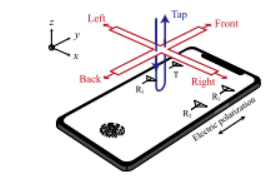
\includegraphics[width=0.75\linewidth]{assets/figs/image.png}
    \caption{手势的定义}
    \label{fig:placeholder}
\end{figure}

\begin{figure}[htbp]
    \centering
    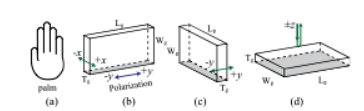
\includegraphics[width=0.75\linewidth]{assets/figs/image1.png}
    \caption{在y极化电场中对手势的调控。（a）手掌。（b） ±x 手势。（c） ±y 手势。（d） ±z 手势。}
    \label{fig:placeholder}
\end{figure}

\subsubsection{错误矫正机制}
在实际应用中，水平手势很容易偏离 $x$- 轴和 $y$- 轴，从而导致潜在的错误判断。为解决此问题，定义了两种冗余手势，即沿对角线方向的手部运动，即 $y = x$ 和 $y = -x$，以最大化容错能力。在实际操作中，一旦识别出手势为对角线运动，则该手势将被判定为无效手势。此类冗余手势消除了 $L$、$R$、$F$ 和 $B$ 手势之间的模糊区域，分别记为 $LF$、$LB$、$RF$ 和 $RB$。

\subsubsection{菲涅耳近场中移动手掌的散射}
在本研究中，使用了一个 $5.8 \text{ GHz}$ 的 $DRS$ 来演示此类手势的识别。在此频率下，对应的波长为 $5.2 \text{ cm}$，与人手的尺寸相当。在这种情况下，人手掌应被视为米氏散射体，且分析应限于菲涅尔近场范围 $[40]$。

\begin{figure}[htbp]
    \centering
    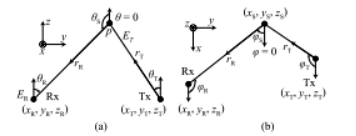
\includegraphics[width=0.75\linewidth]{assets/figs/image2.png}
    \caption{E移动手掌散射分析的双基地模型。（a）yOz 视图。（b）xOy 视图。}
    \label{fig:placeholder}
\end{figure}

为了简化对人体手部米氏散射的分析，我们规定手势将通过平展的手掌执行，如图 3(a) 所示。然后，该手掌可近似为一个导电的扁平长方体，以不同的方向在 $\pm x$、$\pm y$ 和 $\pm z$ 方向上移动。在图 3(b)-(d) 中，长方体的长度、宽度和厚度分别用 $L_g$、$W_g$ 和 $T_g$ 表示。阴影面为面向发射和接收天线的一面。当手掌在水平和垂直方向移动时，长方体的底侧和前面会将大部分入射场散射回接收天线。

在天线理论中，连续表面的散射可被视为来自孔径天线的二次辐射。通常，远场方程（如 $Friis$ 方程）以及线天线的辐射方向图可方便地用于分析此类散射。然而，这些方法在菲涅尔近场中并不适用。

此处采用一种 $ab \ initio$ 方法，通过沿矩形孔径的 $x$- 和 $y$- 方向积分 $y$ 极化赫兹偶极子的辐射，来分析此类近场散射。在图 4 所示的全局 $x$-$y$-$z$ 坐标系统中，假设发射天线和接收天线的相位中心分别位于 $(x_T, y_T, z_T)$ 和 $(x_R, y_R, z_R)$。垂直轴指向 $+z$ 方向。我们还假设散射孔径的几何中心位于 $(x_S, y_S, z_S)$，其垂直轴指向 $+z$ 方向。

从数学上讲，发射天线照射到散射孔径上的电场可表示为
\begin{equation}
\boldsymbol{E}_T(r_T, \theta_T, \varphi_T) = \boldsymbol{\hat{y}} E_0 G_T(\theta_T, \varphi_T) e^{-j k r_T} / r_T
\end{equation}
其中 $G_T(\theta_T, \varphi_T)$ 是发射天线的辐射方向图，$r_T$ 是从发射天线到该单元的距离。类似地，我们将 $G_R(\theta_R, \varphi_R)$ 定义为接收天线的辐射方向图，$r_R$ 为从该单元到接收天线的距离。这里可以使用远场辐射方向图，因为智能设备中使用的四分之一波长倒 $F$ 天线的远场菲涅尔范围较小。

根据图 4 中定义的坐标系，对于散射孔径上偏离 $(x_S, y_S, z_S)$、记为 $(x_S + \zeta, y_S + \xi, z_S)$ 的点，所有坐标系中的仰角、方位角以及距离可以确定为

\begin{equation}
\left\{
\begin{aligned}
\theta_T &= \arctan(\sqrt{(x_S+\zeta-x_T)^2+(y_S+\xi-y_T)^2}/(z_S-z_T)) \\
\varphi_T &= \arctan[(y_S+\xi-y_T)/(x_S+\zeta-x_T)] \\
\theta_S &= \arctan(\sqrt{(x_R-x_S-\zeta)^2+(y_R-y_S-\xi)^2}/(z_R-z_S)) \\
\varphi_S &= \arctan[(y_R-y_S-\xi)/(x_R-x_S-\zeta)] \\
\theta_R &= \arctan(\sqrt{(x_S+\zeta-x_R)^2+(y_S+\xi-y_R)^2}/(z_S-z_R)) \\
\varphi_R &= \arctan[(y_S+\xi-y_R)/(x_S+\zeta-x_R)] \\
r_T &= \sqrt{(x_S+\zeta-x_T)^2+(y_S+\xi-y_T)^2+(z_S-z_T)^2} \\
r_R &= \sqrt{(x_S+\zeta-x_R)^2+(y_S+\xi-y_R)^2+(z_S-z_R)^2}.
\end{aligned}
\right.
\end{equation}

在 $y$ 极化入射光照射下，矩形散射孔径上感应的电流在 $y$ 方向上满足正弦分布 $[40]$。它由沿 $x$ 方向的无限长线电流组成，每个线电流具有如下表面电流分布：

\begin{equation}
J(\zeta, \xi) = I_0 \sin \left[ k \left( \frac{l}{2} - |\xi| \right) \right]
\end{equation}

其中幅度 $I_0 = \sigma_e E_T(r_T, \theta_T, \varphi_T)|_{\zeta=0, \xi=0}$，$\sigma_e$ 为等效电导率。该电流可进一步划分为无限多个 $y$ 极化的赫兹偶极子。对于位于 $(x_S + \zeta, y_S + \xi, z_S)$ 的赫兹偶极子，其 $y$ 分量远场辐射可推导为（见附录）

\begin{equation}
\begin{aligned}
d E_S^y &(\zeta, \xi, r, \theta, \varphi) \\
&= \frac{-j k \eta_0 J(\zeta, \xi) e^{-jkr}}{4 \pi r} (\cos^2 \theta \sin^2 \varphi + \cos^2 \varphi) d\zeta d\xi.
\end{aligned}
\end{equation}

然后，通过沿 $x$- 和 $y$ 方向对所有此类赫兹偶极子的辐射进行积分，可得到矩形孔径散射的总场，接收天线检测到的电场可推导为

\begin{equation}
E_R = \int_{-l/2}^{l/2} \int_{-w/2}^{w/2} G_R(\theta_R, \varphi_R) \cdot d E_S^y(\zeta, \xi, r_R, \theta_R, \varphi_R).
\end{equation}

图 5(a)-(c) 展示了基于 (6) 式在 $20 \text{ cm}$ 的近场菲涅尔距离处计算得到的随 $\theta$ 变化的幅度和相位辐射方向图，分别对应 "左/右"、"后/前" 和 "点击" 手势，其中 $L_g$、$W_g$ 和 $T_g$ 分别为 $15$、$8$ 和 $2 \text{ cm}$。

可以看出，所有幅度图样中的主瓣都较宽，有利于覆盖所有接收天线。在图 5(a) 中，由于 $x$（或 $\varphi = 0/180^\circ, \theta = 90^\circ$）方向上的 $y$ 极化照射，其相位偏移几乎保持恒定，且不受 "左/右" 移动的影响。类似平坦的相位偏移区域也可在图 5(b) 和 (c) 中分别对应于 $\pm y$（或 $\varphi = 90^\circ/-90^\circ, \theta = 90^\circ$）和 $\pm z$（或 $\theta = 0/180^\circ$）方向上找到，它们分别适用于 "前后" 和 "轻触" 手势。如下文所示，这种平坦的相位响应将产生准线性、确定性的多普勒相位，这对 $HGR$ 至关重要。上述手势的定义也正是基于此。

\begin{figure}[htbp]
    \centering
    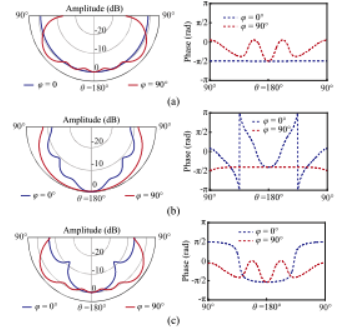
\includegraphics[width=0.75\linewidth]{assets/figs/image3.png}
    \caption{通过(6)式计算的不同孔径尺寸下的散射方向图。(a)w = 2 cm，l = 15cm。(b)w = 15 cm，l = 2 cm。(c)w = 8 cm，l = 15 cm。}
    \label{fig:placeholder}
\end{figure}

\subsubsection{双基地雷达检测到的多普勒信号}
一个单输入多输出（$SIMO$）$DRS$ 可被视为多个共享同一发射通道的双基地雷达的组合。图 6 展示了一个用于检测运动物体的双基地雷达。某物体从 $(x_S, y_S, z_S)$ 位置以速度 $\boldsymbol{v} = (v_x, v_y, v_z)$ 和位移 $\boldsymbol{p} = (p_x, p_y, p_z)$ 移动。径向速度 $\boldsymbol{v}_T$ 和 $\boldsymbol{v}_R$ 是 $\boldsymbol{v}$ 在矢量 $\boldsymbol{r}_T$ 和 $\boldsymbol{r}_R$ 上的投影，因此对应往返距离 $r(t) = |\boldsymbol{r}_T(t)| + |\boldsymbol{r}_R(t)|$。

在一个短时间间隔 $\Delta t$ 内，其中 $\Delta \boldsymbol{p}(t) = (v_x(t), v_y(t), v_z(t)) \Delta t$
\begin{equation}
r(t + \Delta t) = \sqrt{|\boldsymbol{r}_T(t) + \Delta \boldsymbol{p}(t)|^2} + \sqrt{|\boldsymbol{r}_R(t) - \Delta \boldsymbol{p}(t)|^2}.
\end{equation}

然后，$r(t)$ 的导数可计算为（见附录）
\begin{equation}
\begin{aligned}
\frac{dr(t)}{dt} &= \lim_{\Delta t \to 0} \frac{r(t + \Delta t) - r(t)}{\Delta t} = \boldsymbol{v}(t) \cdot \boldsymbol{\hat{r}}_T - \boldsymbol{v}(t) \cdot \boldsymbol{\hat{r}}_R \\
&= |v_T(t)| - |v_R(t)|.
\end{aligned}
\end{equation}

根据多普勒公式 $[41]$, 多普勒频率偏移可计算为
\begin{equation}
f_d(t) = (|v_R(t)| - |v_T(t)|) f_c / c
\end{equation}
其中 $f_c$ 为载波频率，$c$ 为光速。根据 (10) 和 (11)
\begin{equation}
r(t) = -\frac{c}{2 \pi f_c} \int 2\pi f_d(t) dt = -\frac{c}{2 \pi f_c} \Phi(t).
\end{equation}

公式 (12) 显示了往返距离 $r(t)$ 与多普勒信号 $-\Phi(t)$ 之间的等效关系。

\begin{figure}
    \centering
    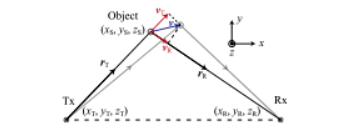
\includegraphics[width=0.75\linewidth]{assets/figs/image5.png}
    \caption{双基地DRS检测到的多普勒相位}
    \label{fig:placeholder}
\end{figure}

\subsubsection{由 $\Phi(t)$ 携带的确定性多普勒信号}
对于图2中布置的天线$T$、$R_1$、$R_2$，和$R_3$，我们假设它们的坐标分别为$(-a, a, 0)$、$(a, a, 0)$、$(a, -a, 0)$和$(-a, -a, 0)$，一个 "向右" 手势在 $z = h$ 平面上移动。其轨迹可描述为 $X(x_g, y, h)$，其中$x_g$ 是该手势散射相位中心的$x$坐标，$y$ 是该手势恒定的$y$坐标。发射器、移动手势与 $TDM$ 接收器之间的往返距离可表示为

\begin{equation}
\left\{
\begin{aligned}
r_1 &= \sqrt{(x_g+a)^2+(y-a)^2+h^2} \\
    &\quad + \sqrt{(x_g-a)^2+(y-a)^2+h^2} \\
r_2 &= \sqrt{(x_g+a)^2+(y-a)^2+h^2} \\
    &\quad + \sqrt{(x_g-a)^2+(y+a)^2+h^2} \\
r_3 &= \sqrt{(x_g+a)^2+(y-a)^2+h^2} \\
    &\quad + \sqrt{(x_g+a)^2+(y+a)^2+h^2}.
\end{aligned}
\right.
\end{equation}

根据$(12)$和$(13)$，可以计算出相应的多普勒信号$-\Phi_i(t)$，如图7所示，其中$i = 1, 2, 3$。可以看出，对于 "向右" 手势，$-\Phi_3(t)$ 的最小值首先出现，随后是$-\Phi_1(t)$ 和$-\Phi_2(t)$ 的最小值。对于位于正方形角落的天线，$-\Phi_1(t)$ 和$-\Phi_2(t)$ 的最小值将同时出现。这种确定但不同的多普勒信号也出现在其他手势中。在本研究中，将利用$-\Phi_i(t)$ 的这些最小值的时间顺序来进行鲁棒的手势识别。
\begin{figure}
    \centering
    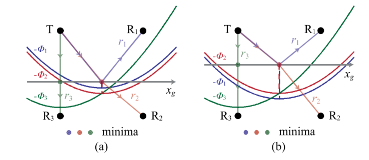
\includegraphics[width=0.75\linewidth]{assets/figs/image6.png}
    \caption{TDM\text{-} SIMO DRS在"向右"手势中检测到的多普勒信号变化。计算中，a = 2.5 cm，h = 10 cm，xg 表示手势从–4.5移动到4.5 cm，y1 和y2 是"向右"手势的y 坐标，在示例中(a) y1 = –0.5 cm，(b) y2 = 0.5 cm。}
    \label{fig:placeholder}
\end{figure}

在$(13)$中，$h$ 也表示手势的高度。当 $h$ 发生变化时，$-\Phi_i(t)$ 曲线的形状也会改变。然而，极小值的时间顺序将保持不变。这意味着基于此类极小值时间顺序的手势识别将与手势的高度无关。

\subsubsection{检测信号的分割}
为了识别预定义的手势，应首先分离包含所有运动信息的信号，即 $\Phi[n]$。这可以通过对检测到的 $I/Q$ 信号进行动态功率分析来实现。
\begin{figure}[htbp]
    \centering
    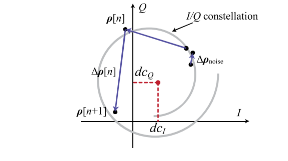
\includegraphics[width=0.75\linewidth]{assets/figs/image7.png}
    \caption{ρ[n] 和  ρnoise 在I/Q 星座图中的示意图。}
    \label{fig:placeholder}
\end{figure}

图 8 说明了采样时刻 $I/Q$ 信号在 $n$ 和 $n + 1$ 处的情况。相邻采样期间 $I/Q$ 信号的变化向量 $\Delta \boldsymbol{\rho}[n]$ 表示。当存在移动散射体时，

\begin{equation}
\Delta \boldsymbol{\rho}[n] =
\begin{pmatrix}
A_I[n+1] \cos(\Phi[n+1]) - A_I[n] \cos(\Phi[n]) + \Delta n_I[n] \\
A_Q[n+1] \sin(\Phi[n+1]) - A_Q[n] \sin(\Phi[n]) + \Delta n_Q[n]
\end{pmatrix}^T
\end{equation}

反映 "$I/Q$" 信号的 "差分功率" $\Delta P[n]$ $I/Q$ 信号的 $\Delta$，其中 $\Delta n_I[n]$ 为 $n_I[n+1] - n_I[n]$，因此 $\Delta n_Q(t)$ 也是如此。这里，$\Delta P[n]$ 可计算为

\begin{equation}
\Delta P[n] = |\Delta \boldsymbol{\rho}[n]|^2.
\end{equation}

在没有任何运动的情况下，$\Delta \boldsymbol{\rho}_{\text{noise}}[n] = (\Delta n_I[n], \Delta n_Q[n])$ 表示电路噪声的 "差分功率"。显然，$\Delta \boldsymbol{\rho}$ 始终大于 $\Delta \boldsymbol{\rho}_{\text{noise}}$，因此 $\Delta P$ 可有效地用于将包含手势信息的信号段与检测到的信号分离。

为确定分割的阈值，可基于 $\Delta \boldsymbol{\rho}_{\text{noise}}$ 的数学期望即 $\text{E}(\Delta \boldsymbol{\rho}_{\text{noise}})$ 来确定，据此可选择略大于该期望的值作为阈值。在本研究中，该值为 $1.1 \ \text{E}(\Delta \boldsymbol{\rho}_{\text{noise}})$。

为了确保分离的可靠性，可以在每个时间间隔对 $\Delta P[n]$ 执行 $m$ 点移动平均窗口处理，其中

\begin{equation}
\overline{\Delta P_m}[n] \triangleq m^{-1} \sum_{j=n-m/2+1}^{n+m/2} \Delta P[j]
\end{equation}

以减少由于意外故障导致的潜在误判。如果 $\overline{\Delta P_m}[n]$ 大于阈值，则认为在此时间间隔内存在运动。所有此类连续的时间间隔对应一个信号段，在该信号段期间被认为存在运动。对所有接收通道检测到的信号均可执行相同的操作。所获得三个信号段反映了从不同方向检测到的同一运动。这些信号段的并集将产生一个最宽的信号段，包含完整运动的信息，从中可以识别出潜在的手势。

\subsubsection{TDM采样的数据对齐}
如图 1 所示，$TDM$-$SIMO$ 架构显著降低了 $DRS$ 的复杂性和成本。然而，采样得到的数据序列需要进行对齐。

对于 $M$ 个 $TDM$ 接收通道，检测到的串行 $I$ 通道序列 $I_1[n], I_2[n+1/M], \dots, I_M[n+(M-1)/M], I_1[n+1], I[+1]n_{2[/M+1+1 \dots]}$ 应重新对齐为 $I_{1,n}, I_{2,n}, \dots, I_{M,n}, I_{1,n+1}, I_{2,n+1}, \dots$。第 $i$ 个通道中，检测信号与对齐信号之间的差异为 $(i-1)T+1/M$，其中 $T_{TDM}$ 是相邻 $TDM$ 采样之间的时间间隔。在本研究中，设计了一组数字相移滤波器 $_{TDM}$ 来补偿这种时间不同步，从而可得到第 $i$ 个通道该滤波器的 $z$ 域响应为 $[42]$。其频率响应为

\begin{equation}
H_i(e^{j\omega}) = H_i(z)|_{z=e^{j\omega}} = e^{j(i-1)\omega/M}
\end{equation}

这种全通相位偏移滤波器可以被综合为

\begin{equation}
\begin{aligned}
h_i(n) &= \frac{1}{2\pi} \int_{-\pi}^{\pi} e^{j(i-1)\omega/M} e^{j\omega n} d\omega \\
&= \frac{\sin\{\pi[n + (i - 1)/M]\}}{\pi[n + (i - 1)/M]}.
\end{aligned}
\end{equation}

将 $I_i[n]$ 与 $h_i(n)$ 进行卷积后，来自不同通道的采样数据可以对齐。类似地，检测到的 $Q$ 通道信号也可以对齐。

\subsubsection{分段收拾的重缩放与拟合}
在完成分割和数据对齐之后，可以获得连续的时间段，每段包含一个单一的手势。对于最宽的手势段，其实际持续时间或总采样数因手势而异。此外，检测到的原始多普勒相位信号 $\Phi_i$ 可能是锯齿状的，因此需要对手势分段信号进行重缩放和拟合，以获得长度一致且形状平滑的规范化手势信号，便于后续识别。

在本研究中，所有最宽的段均被重缩放至 $(0, 1)$ 区间。为了保持 $-\Phi_i$ 的形状并防止毛刺的影响，本文采用八阶多项式拟合，从而使信号 $-\Phi_i$ 上的噪声不会被拟合。

在重缩放和拟合之后，第 $i$ 个通道的 $-\Phi_i$ 极小值时刻（如 II-E 节所述）可在区间 $(0, 1)$ 内量化，并表示为 $t_{m,i}$。在本研究中，极小值时刻以向量形式表示为 $\boldsymbol{t}_m = (t_{m,1}, t_{m,2}, t_{m,3})$，可用于表征每种手势，并将作为后续讨论的分类器的输入。

经过此次重缩放后，极小值时刻与手势速度无关。这在识别快速和慢速手势方面起着重要作用。

\subsubsection{基于分类的手势识别}

分类是机器学习中常用的技术之一 $[23]$，旨在将一组数据进行分类到各个类别中。它已应用于图像识别、语音处理、生物信息学、自然语言处理等领域 $[24]$。

迄今为止，已有多种分类算法或分类器被提出。主流分类器包括逻辑回归、线性判别分析（$LDA$）、决策树、朴素贝叶斯分类器和支持向量机（$SVM$）$[43]$。

在本研究中，选择用于多分类的一对多（$OVR$）$SVM$ 来识别预定义的多类手势。信号处理、基于已知手势数据集训练 $OVR \ SVM$ 以及对未知手势进行识别的流程图分别如图 $9(a)$-$(c)$ 所示。

为了训练 $OVR \ SVM$，可以通过对每个已定义的手势检测 $N$ 次来准备包含已知手势的数据集。然后，该数据集可复制成 $C$ 份，其中 $C$ 为已定义手势的数量。在第 $i$ 个 $SVM$ 的训练中，所有第 $i$ 个手势被标记为 $+1$，其余所有手势均被标记为 $-1$。

基于训练好的 $SVM$，可通过比较每个 $SVM$ 评估出的 "得分" 或相似度来识别新手势。如果第 $i$ 个 $SVM$ 给出的得分最高，则该手势将被识别为第 $i$ 个手势。更多细节见 $[23]$。

\subsection{仿真}
为了验证第三节中提出方法的有效性，我们根据图 9 所示的步骤，基于推导出的方程进行了数值仿真。在所有仿真中，发射天线和接收天线 $T$、$R_1$、$R_2$ 和 $R_3$ 的坐标分别为 $(-2.5, 2.5, 0)$、$(2.5, 2.5, 0)$、$(2.5, -2.5, 0)$ 和 $(-2.5, -2.5, 0)$；简化手掌模型的 $L$、$W$ 和 $T$ 分别为 $15$、$8$ 和 $2$，单位均为厘米。
\begin{figure}[htbp]
    \centering
    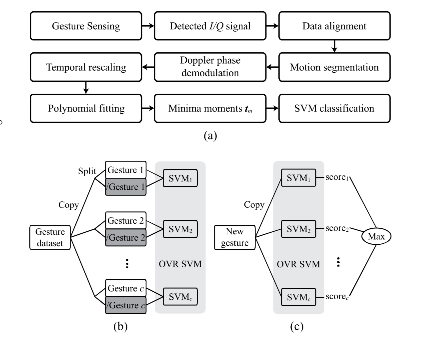
\includegraphics[width=0.75\linewidth]{assets/figs/image8.png}
    \caption{手势识别流程图。（a）信号处理。（b）OVR SVM 的训练。（c）基于已
训练 OVR SVM 的手势识别。}
    \label{fig:placeholder}
\end{figure}

\subsubsection{不同手掌方向检测到的多普勒信号}
定义的手势可分为两种类型。对于"左"、"右"、
"前"、"后"和"对角"手势，手掌垂直于天线平面，以较窄的孔径散射照射场。对于"轻触"手势，手掌平行于天线平面，以大得多的孔径进行散射。

为解释定义这两类手势的原因，我们比较了手掌垂直和平行时执行"右"手势所计算出的多普勒信号。在计算中，两个散射孔径中心即 $(X_S, y, h)$ 分别从 $(-20, 0, 10)$ 移动到 $(20, 0, 10)$。根据公式 $(2)$-$(8)$，$I/Q$ 信号的星座图、差分功率 $\Delta P[n]$，以及恢复的多普勒相位 $-\Phi[n]$，如图 $10$ 所示。

可以看出，垂直和平行移动的手掌会产生非常不同的 $I/Q$ 信号和多普勒相位。特别是对于平行移动的手掌，图 $10(c)$ 中的极小值几乎无法确定，而图 $10(f)$ 中的极小值则很容易识别。这正是定义在天线平面上方平行移动手势时所考虑的因素。

\subsubsection{按照流程图进行仿真}
在本节中，将按照图 9(a) 所示步骤进行数值仿真。
\begin{figure}[htbp]
    \centering
    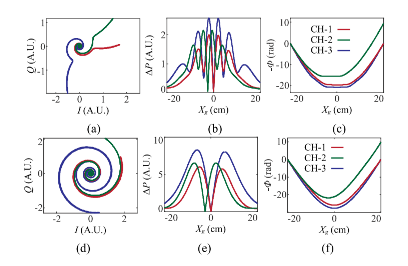
\includegraphics[width=0.75\linewidth]{assets/figs/image9.png}
    \caption{针对掌心不同朝向模拟生成的多普勒信号。（a）–（f）分别为
I/Q 信号的星座图、分段后的差分功率以及平行和垂直掌心情况下恢复
的多普勒相位。}
    \label{fig:placeholder}
\end{figure}

首先，使用与计算图 10 相同的方法，也可以计算出由 $R_1, R_2, \text{和} R_3$ 天线分别 "检测" 到的两个连续的 "向右" 和 "向左" 手势所产生的 $I/Q$ 信号。结果如图 11 所示。不同之处在于添加了白高斯噪声，使得 $I/Q$ 信号能够在 $20 \text{ dB}$ 信噪比（$SNR$）下生成。
\begin{figure}[htbp]
    \centering
    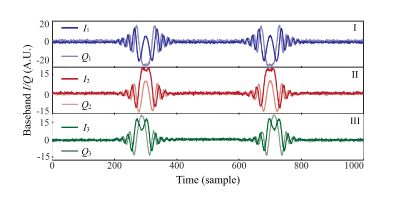
\includegraphics[width=0.75\linewidth]{assets/figs/image10.png}
    \caption{由R1, R2, 和R3 天线分别"检测"到的两个连续"向右"和"向左"手势所
产生的模拟I/Q 信号。}
    \label{fig:placeholder}
\end{figure}

然后，根据第三节-F 对这些信号进行分段。图 12 中的面板 I 和 II 分别显示了解调后的多普勒相位以及 $60$ 点移动平均微分功率 $\Delta P_{60}[n]$。选择阈值为 $2$ 时，手势可以在灰色标记的区域中被分割。可以看出，两个手势都被正确地分割。面板 III 展示了在更差的 $10 \text{ dB}$ 信噪比条件下与面板 II 相同的计算结果。可以看出，手势片段几乎无法识别。
\begin{figure}[htbp]
    \centering
    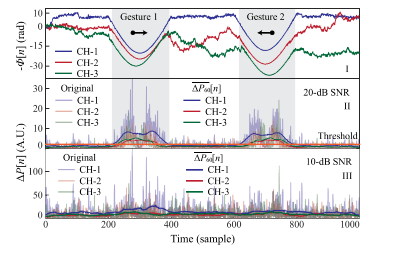
\includegraphics[width=0.75\linewidth]{assets/figs/image11.png}
    \caption{两个连续"向右"和"向左"手势的分段结果。子图I：20 dB
SNR下的解调多普勒相位。子图II：20 dB SNR下模拟基带信号的 P[
n] 和P60[n] ，以及用于分段的阈值。子图III：10 dB SNR下模拟基带信
号的 P[n] 和 P60[n] 。}
    \label{fig:placeholder}
\end{figure}

接下来，基于第三节-H 的讨论，通过八阶多项式拟合对已分割的手势进行重缩放。如图 13 所示，在重缩放和拟合之后，可以清晰提取重缩放后多普勒相位的极小值时刻，并据此确定这些极小值的时间顺序。在本研究中，这种在通道顺序上确定且量化的极小值，例如该图中的 $\boldsymbol{t}_m = (0.48, 0.48, 0.42)$ 和 $\boldsymbol{t}_m = (0.47, 0.47, 0.54)$，被用作 $OVR \ SVM$ 分类器的输入，而不是 "黑箱" 手势分类中使用的 $I/Q$ 星座图或多普勒特征。
\begin{figure}[htbp]
    \centering
    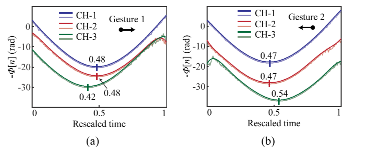
\includegraphics[width=0.75\linewidth]{assets/figs/image12.png}
    \caption{连续"右"和"左"手势的缩放并拟合后的多普勒相位中多普勒极
小值的确定。深色线条：八阶多项式拟合的多普勒相位。浅色线条：含
噪声的原始多普勒相位。(a) 手势1的量化极小值时刻为tm = (0.48,
0.48, 0.42)，(b) 手势2的量化极小值时刻为tm = (0.47, 0.47, 0.54)。}
    \label{fig:placeholder}
\end{figure}

\begin{figure}[htbp]
    \centering
    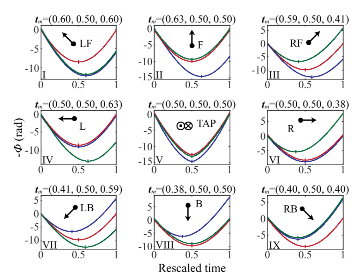
\includegraphics[width=0.75\linewidth]{assets/figs/image13.png}
    \caption{不同接收通道检测到的定义手势的模拟多普勒相位。}
    \label{fig:placeholder}
\end{figure}

图 14 显示了从为所有定义的手势模拟的 $I/Q$ 信号中分割出的多普勒相位。在仿真中，对于所有水平方向移动的手势，手底边与天线平面之间的距离设为 $10 \text{ cm}$；对于敲击手势，手掌与天线平面之间的最短距离设为 $5 \text{ cm}$。可以看出，每个分割手势的极小值的时间序列顺序是确定的。

\subsection{实验}
\subsubsection{时分双工单输入多输出DRS的实现}
\begin{figure}[htbp]
    \centering
    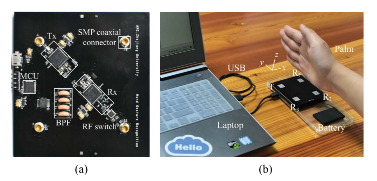
\includegraphics[width=0.75\linewidth]{assets/figs/image14.png}
    \caption{使用一对 Wi\text{-}Fi 芯片实现的时分双工单输入多输出 DRS。（a）射频板。
（b）电池供电的 DRS 及实验环境。}
    \label{fig:placeholder}
\end{figure}
图 15 展示了根据图 1 提出架构实现的 $TDM$-$SIMO \ DRS$。在本研究中，使用了一对 $Wi$-$Fi$ 芯片 $Maxim \ Integrated \ MAX2829$ 来模拟 $5.8 \text{ GHz}$ 的 $LTE$-$U$ 和 $Wi$-$Fi$ 信道，并使用射频开关 $HMC7992$ 将接收信道分别切换至天线 $R_1, R_2, \text{和} R_3$。类似于 $[44]$, 采用 $L$ 形排列的接收天线用于检测三维手势。在不失一般性的前提下，这些天线被设计为标准贴片天线。天线板与射频板通过四个超小型推入式连接器（$SMP$）同轴连接器相连。一个标准锂电池为 $DRS$ 供电。采用 $STM32F103T8U6$ 微控制器单元（$MCU$）对 $Wi$-$Fi$ 芯片进行配置，并通过 $MCU$ 内置的 $ADC$ 采集 $I/Q$ 信号。采样数据最终通过安装在射频板上的 $Silicon \ Labs \ CP2102$ 通用串行总线（$USB$）-通用异步收发传输器（$UART$）桥接芯片传输到笔记本电脑。

\subsubsection{实验手势信号的处理}
\begin{figure}[htbp]
    \centering
    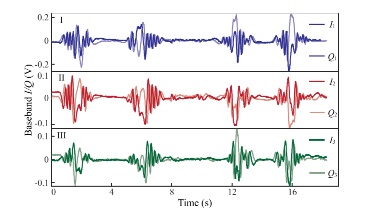
\includegraphics[width=0.75\linewidth]{assets/figs/image15.png}
    \caption{实验 I/Q 信号来自天线 R1, 、R2, 和 R3, 分别检测到的连续四次
"向前"、"向后"、"向左"和"向右"手势。}
    \label{fig:placeholder}
\end{figure}

\begin{figure}[htbp]
    \centering
    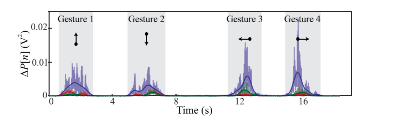
\includegraphics[width=0.75\linewidth]{assets/figs/image16.png}
    \caption{基于图16中检测到的信号的微分功率 P[n] 以及移动平均P60[n]
进行的分割过程。}
    \label{fig:placeholder}
\end{figure}

\begin{figure}[htbp]
    \centering
    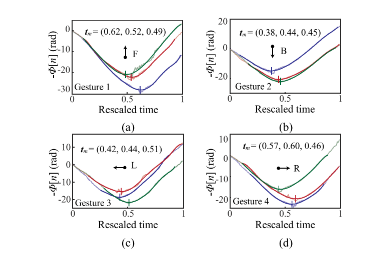
\includegraphics[width=0.75\linewidth]{assets/image.png}
    \caption{图16中连续四个手势的重缩放并拟合后的多普勒相位多普勒极小值
的确定。深色线条：八阶多项式拟合的多普勒相位曲线。浅色线条：原
始多普勒相位曲线。四个手势的量化极小值时刻分别为(0.62, 0.52,
0.49)、(0.38, 0.44, 0.45)、(0.42, 0.44, 0.51)和(0.57, 0.60, 0.46)。}
    \label{fig:placeholder}
\end{figure}

\begin{figure}[htbp]
    \centering
    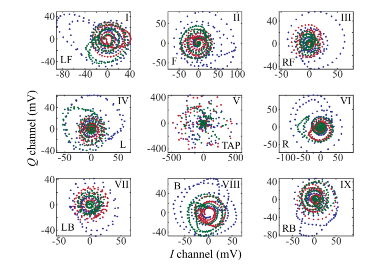
\includegraphics[width=0.75\linewidth]{assets/image0.png}
    \caption{实验中执行手势的星座图。}
    \label{fig:placeholder}
\end{figure}

对应于图 11-13，图 16 中的面板 I-III 分别显示了天线 $R_1, R_2, \text{和} R_3$ 检测到的基带 $I/Q$ 信号，依次对应连续的 "前"、"后"、"左" 和 "右" 手势。采用相同的处理方法计算得到图 12 和图 17，展示了图 16 中检测到的手势分割结果。图 18 显示了经解调后的多普勒相位及其极小值时刻 $t_m$，以便进一步分类。

可以看出，对于实验数据，以 "向右" 手势为例，由于实际手部的非平面散射孔径，$-\Phi_1(t)$ 和 $-\Phi_2(t)$ 的最小值可能出现的时间略有不同。然而，如果用于训练分类器的数据集包含了此类偏移的最小值，则其对分类的准确性影响较小。

对应于图 14，相同九种手势在距离天线平面相同距离处执行，$TDM$-$SIMO \ DRS$ 检测到的这些手势对应的 $I/Q$ 信号星座图分别如图 19 所示。可以注意到，由于手掌的垂直运动和更大的散射面积，"点击" 手势的幅度和形状与其他手势明显不同。
\begin{figure}[htbp]
    \centering
    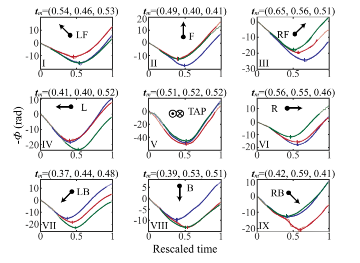
\includegraphics[width=0.75\linewidth]{assets/image1.png}
    \caption{执行手势的实验多普勒相位变化及极小值时刻。}
    \label{fig:placeholder}
\end{figure}
图 20 显示了从图 19 绘制的星座图中检索出的 $-\Phi_i$。可以看出，极小值点的顺序 $t_m$ 与图 14 中的顺序一致。

\subsubsection{手势分类}
为了对定义的手势进行分类，我们为不同的手势收集了500个样本作为数据集，每个手势50到60个样本。其中，500个样本中的80\%（每个手势约40到50个样本）被随机选作训练集。剩余的20\%被选作测试集，包括待识别的未知手势。为了可视化训练集和测试集中的极小值时刻$t_m$，建立了一个矩形坐标系，其坐标轴对应于每个接收通道检测到的极小值时刻。如图 21 所示，在两个数据集中，每种手势的极小值时刻均被聚类，并且与其他聚类明显分离，验证了由极小值时刻表示的手势具有确定性。这也意味着，使用训练集训练得到的 $OVR \ SVM$ 可以准确分类测试集中的手势。
\begin{figure}[htbp]
    \centering
    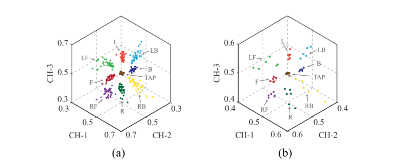
\includegraphics[width=0.75\linewidth]{assets/image2.png}
    \caption{将各类手势的多普勒相位极小值时刻tm 映射到三维特征坐标系中。
坐标轴表示通道1–3的重缩放时间。(a) 训练集。(b) 测试集。}
    \label{fig:placeholder}
\end{figure}

\begin{figure}[htbp]
    \centering
    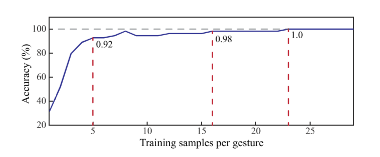
\includegraphics[width=0.75\linewidth]{assets/image3.png}
    \caption{通过未知样本评估的OVRSVM学习曲线。}
    \label{fig:placeholder}
\end{figure}

为了评估基于极小值时刻分类的鲁棒性，我们通过使用不同子集训练得到的 $OVR \ SVM$ 对 $50$ 个未知手势进行分类，计算出学习曲线 $[23]$。结果如图 22 所示。可以看出，仅用六个样本训练的 $OVR \ SVM$ 即可达到 $98\%$ 的识别准确率，当训练样本增加到 $23$ 个时，可获得 $100\%$ 的准确率。使用普通个人计算机进行训练耗时不到 $3 \text{ s}$。

为了验证该分类器的泛化能力，通过邀请另外四名受试者执行相同的 $gesture$ 进行了一次留一受试者实验 $[12]$。每个手势重复 $10$ 次。在执行之前，他们了解每个手势的移动方向、手部姿势以及敏感区域。图 23 显示了由这些受试者检测到的极小值时刻组成的数据集的映射情况。可以看出，与图 21(a) 所示训练集的映射相比，这些极小值时刻也呈现出聚类且明显分离的状态。这表明，尽管不同受试者执行的手势之间存在差异，但经过重新缩放的极小值时刻对于 $OVR \ SVM$ 分类器而言仍表现出足够的相似性。

使用基于原始受试者检测数据集训练的分类器，对图 23 中其他受试者检测到的最小动作时刻进行分类。通过计算每个新受试者的混淆矩阵，可分别获得 $96.67\%$、$100\%$、$97.78\%$ 和 $96.67\%$ 的识别准确率，该结果验证了由某一特定受试者训练得到的分类器适用于未知受试者。
\begin{figure}[htbp]
    \centering
    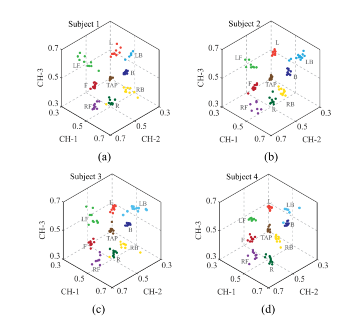
\includegraphics[width=0.75\linewidth]{assets/image4.png}
    \caption{从新受试者检测到的最小值时刻的映射。}
    \label{fig:placeholder}
\end{figure}

\begin{figure}[htbp]
    \centering
    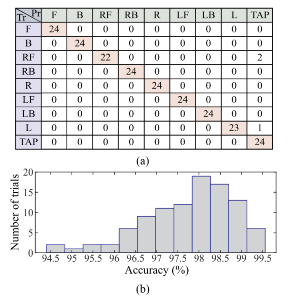
\includegraphics[width=0.6\linewidth]{assets/image5.png}
    \caption{. 训练后的 OVR SVM 准确性评估。（a）混淆矩阵，其中 Tr 和 Pr 分
别代表"真实"和"预测"。（b）100 次试验中交叉验证准确率的直方图。}
    \label{fig:placeholder}
\end{figure}

最后进行了交叉验证 $[23]$ 实验，其中将来白全部五名受试者的检测手势混合在一起。在混合的手势中，随机选择 $75\%$ 的手势作为训练集，其余 $25\%$ 作为测试集。对于每种手势，测试集中的手势数量为 $24$ 个。图 24 显示了针对参与单个受试者留出实验的五名受试者所执行手势计算得到的混淆矩阵。可计算得出，总体识别准确率高达 $98.6\%$。此外，图 24(b) 展示了 $100$ 次试验中交叉验证准确率的直方图。经计算，最大、最小和平均准确率分别为 $99.54\%$、$94.44\%$ 和 $97.83\%$，标准差为 $1.15\%$。

\begin{figure}[htbp]
    \centering
    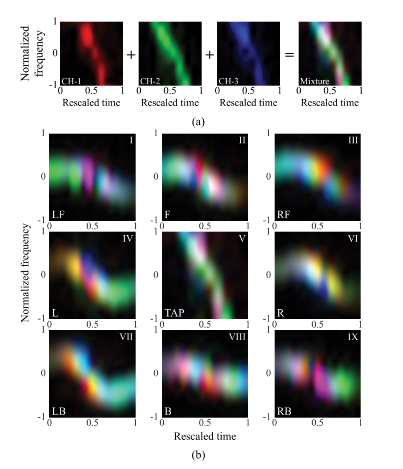
\includegraphics[width=0.6\linewidth]{assets/image6.png}
    \caption{不同手势产生的时频谱图。（a）单色和全色谱图。（b）用于基
于 DCNN 分类的全色多普勒谱图。}
    \label{fig:placeholder}
\end{figure}

\subsubsection{讨论}
上述结果验证了所提出的基于检测和处理确定性多通道多普勒信号的智能设备方法的有效性和准确性。

作为消费产品，智能手机等智能设备高度集成、紧凑，并且对电池寿命、产品尺寸和成本极为关注。该连续波解决方案工作在单一频率，可通过重用智能设备现有的射频资源来实现，增加的成本、功耗和空间占用均可忽略不计。

多普勒信号的确定性带来了一个独特特征，即使用极小数据集训练的高效 $OVR \ SVM$ 分类器即可实现高识别准确率。相比之下，基于对多普勒信号时频谱进行分类的手势识别则需要多得多的训练样本。

作为对比，图 $25(a)$ 展示了 $SIMO \ DRS$ 每个通道检测到的多普勒相位的短时傅里叶变换（$STFT$）。在计算该 $STFT$ 谱图时，对每个通道使用了 $20$ 点的汉宁滑动窗，重叠点数为 $10$。由于每个手势的时间持续长度不同，因此将谱图调整为 $400 \times 400$ 像素。然后，将每个通道的谱图强度归一化到 $(0, 1)$ 范围内。

将获得的时频谱绘制成单色红、绿、蓝三色图像，然后混合生成全色 $spectrogram$。图 $25(b)$展示了基于图 19 所示信号计算出的九种不同手势的 $spectrogram$。在以往基于多普勒雷达的识别 $[10], [12], [14], [16], [17], [25]$ 中，此类 "图像" 被用于训练分类器，通常为深度卷积神经网络（$DCNN$），之后可通过训练好的 $DCNN$ 识别未知手势。
\begin{figure}[htbp]
    \centering
    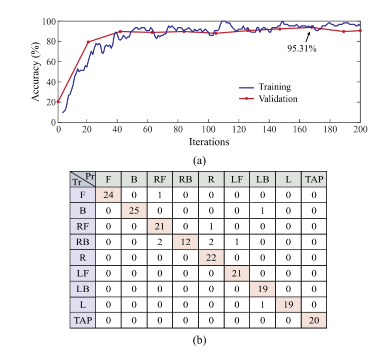
\includegraphics[width=0.75\linewidth]{assets/image01.png}
    \caption{与基于DCNN分类的比较。（a）DCNN分类器的训练。（b）混淆矩阵。}
    \label{fig:placeholder}
\end{figure}

例如，使用检测到的手势的 $560$ 个频谱图来训练适用于移动和嵌入式设备的 "$MobileNets$" $DCNN \ [45]$，并采用大小为 $8$ 的小批量以避免潜在的过拟合。这些频谱图来自全部五名受试者的混合样本。然后，通过训练好的 $DCNN$ 对 $192$ 个未知频谱图进行分类，从而获得识别准确率随迭代次数的变化情况。

如图 $26(a)$ 所示，随着迭代次数的增加，识别准确率总体呈上升趋势。最终的识别准确率达到 $95.31\%$。在普通计算机上，基于频谱图训练 $DCNN$ 耗时约 $8$ 分钟，远长于基于序列极小值矩训练 $OVR \ SVM$ 所用的 $3$ 秒。尽管 $DCNN$ 需要更大的训练集，但其难以达到 $100\%$ 的识别准确率。基于训练好的 $DCNN$，可计算出如图 $26(b)$ 所示的混淆矩阵。

实际手势识别的另一个挑战是处理干扰性的随机手势和动作。在本研究中，尽管 $OVR \ SVM$ 能够帮助过滤掉其中一部分，但该问题主要在信号分割阶段得以解决。如图 $20$ 所示，对于每一个符合条件的手势，由于每个接收天线检测到的多普勒相位分割曲线是凸函数，因此仅存在一个最小值时刻。因此，只需检查分割信号中最小值时刻的数量，即可排除随机手势或动作。

最后，本研究所定义的手势对应于多点触控屏幕的主
要功能，目的是为智能设备提供额外的无线手势控制功能。
这些手势的多普勒相位曲线均为凸函数。我们的方法也可
扩展至双向和多向手势，其多普勒相位曲线由多个相连的
凸函数组成。这类手势可以是在水平面或垂直面内执行的
手势组合。然而，现有方法不适用于无法提取出有序最小
值时刻的手势。对于诸如手指摩擦等手势，基于微多普勒
的分析可能是必不可少的。

\subsection{结论}
总之，我们从理论上分析并实验验证了基于单输入多输出差分雷达系统（$SIMO$-$DRS$）的手势识别方法，该方法可通过轻微修改智能设备现有的射频前端来实现。通过检测和处理由 $SIMO$ 雷达系统探测到的确定性多普勒信号，仅需少量数据集即可训练一个 $OVRSVM$，并实现九种预定义手势的毫秒级识别。我们设想这种鲁棒且高效的方法还可扩展到多种应用中。

\subsection{附录}
\subsubsection{公式(7)的推导}
对于一个y极化的赫兹偶极子，记其矢量势为

\begin{equation}
\boldsymbol{A} = \boldsymbol{\hat{y}} \mu I \Delta l e^{-jkr} / 4 \pi r
\end{equation}

其中 $\Delta l$ 和 $I$ 分别为无穷小长度和线电流强度。在 $r$-$\theta$-$\varphi$ 球坐标系中

\begin{equation}
\boldsymbol{\hat{y}} = \boldsymbol{\hat{r}} \sin \theta \sin \varphi + \boldsymbol{\hat{\theta}} \cos \theta \sin \varphi + \boldsymbol{\hat{\varphi}} \cos \varphi
\end{equation}

然后，电场

\begin{equation}
\begin{aligned}
\boldsymbol{E} &= \frac{1}{j \omega \varepsilon} \nabla \times \boldsymbol{H} = \frac{1}{j \omega \varepsilon} \nabla \times \left( \frac{1}{\mu} \nabla \times \boldsymbol{A} \right) \\
&= \frac{1}{j \omega \varepsilon} \frac{I \Delta l}{4 \pi} \left[ \frac{2}{r^3} (1 + jkr) \sin \theta \sin \varphi e^{-jkr} \boldsymbol{\hat{r}} \right. \\
&\quad + \left( \frac{k^2}{r} - \frac{1}{r^3} - \frac{jk}{r^2} \right) \cos \theta \sin \varphi e^{-jkr} \boldsymbol{\hat{\theta}} \\
&\quad \left. + \left( \frac{k^2}{r} - \frac{1}{r^3} - \frac{jk}{r^2} \right) \cos \varphi e^{-jkr} \boldsymbol{\hat{\varphi}} \right]
\end{aligned}
\end{equation}

在远场区域

\begin{equation}
\begin{aligned}
\lim_{r \to \infty} \boldsymbol{E} &= \frac{1}{j \omega \varepsilon} \frac{I \Delta l}{4 \pi} \frac{k^2}{r} e^{-jkr} (\boldsymbol{\hat{\theta}} \cos \theta \sin \varphi + \boldsymbol{\hat{\varphi}} \cos \varphi) \\
&= \frac{-j k \eta_0 I \Delta l e^{-jkr}}{4 \pi r} (\boldsymbol{\hat{\theta}} \cos \theta \sin \varphi + \boldsymbol{\hat{\varphi}} \cos \varphi)
\end{aligned}
\end{equation}

在直角坐标系中

\begin{equation}
\begin{aligned}
\boldsymbol{\hat{\theta}} &= \boldsymbol{\hat{x}} \cos \theta \cos \varphi + \boldsymbol{\hat{y}} \cos \theta \sin \varphi - \boldsymbol{\hat{z}} \sin \theta \\
\boldsymbol{\hat{\varphi}} &= -\boldsymbol{\hat{x}} \sin \varphi + \boldsymbol{\hat{y}} \cos \varphi
\end{aligned}
\end{equation}

那么，赫兹偶极子散射的电场的y分量为

\begin{equation}
E_{dipole}^y = \frac{-jk\eta I \Delta l e^{-jkr}}{4\pi r}(\cos^2 \theta \sin^2 \varphi + \cos^2 \varphi)
\end{equation}

将 $I \Delta l$ 替换为实际的表面电流元 $J(\zeta, \xi)d\zeta d\xi$，该赫兹偶极子辐射的远场电场可推导为

\begin{equation}
\begin{aligned}
d E_S^y &(\zeta, \xi, r, \theta, \varphi) \\
&= \frac{-j k \eta_0 J(\zeta, \xi) e^{-j k r}}{4 \pi r} (\cos^2 \theta \sin^2 \varphi + \cos^2 \varphi) d \zeta d \xi.
\end{aligned}
\end{equation}

\subsubsection{公式(9)和(10)的推导}
对于图 6 所述的双基地雷达，瞬态位移 $\boldsymbol{p} = (p_x, p_y, p_z)$ 和三维瞬态速度 $\boldsymbol{v} = (v_x, v_y, v_z)$ 满足 $\boldsymbol{v} = d \boldsymbol{p}/dt$，其微分形式是 $\Delta \boldsymbol{p}(t) = \boldsymbol{v}(t) \Delta t$。因此，往返距离在时间 $t$ 和 $t + \Delta t$ 时可分别计算为 $r(t) = |\boldsymbol{r}_T(t)| + |\boldsymbol{r}_R(t)|$ 和

\begin{equation}
r(t + \Delta t) = \sqrt{|\boldsymbol{r}_T(t) + \Delta \boldsymbol{p}(t)|^2} + \sqrt{|\boldsymbol{r}_R(t) - \Delta \boldsymbol{p}(t)|^2}
\end{equation}

当 $\Delta t$ 趋近于 $0$ 时

\begin{equation}
\begin{aligned}
\lim_{\Delta t \to 0} &r(t + \Delta t) \\
&= \lim_{\Delta t \to 0} \sqrt{|\boldsymbol{r}_T(t)|^2 + 2 \boldsymbol{r}_T(t) \cdot \Delta \boldsymbol{p}(t) + |\Delta \boldsymbol{p}(t)|^2} \\
&\quad + \sqrt{|\boldsymbol{r}_R(t)|^2 - 2 \boldsymbol{r}_R(t) \cdot \Delta \boldsymbol{p}(t) + |\Delta \boldsymbol{p}(t)|^2} \\
&\approx \lim_{\Delta t \to 0} \sqrt{|\boldsymbol{r}_T(t)|^2 + 2 \boldsymbol{r}_T(t) \cdot \Delta \boldsymbol{p}(t)} \\
&\quad + \sqrt{|\boldsymbol{r}_R(t)|^2 - 2 \boldsymbol{r}_R(t) \cdot \Delta \boldsymbol{p}(t)} \\
&\approx \lim_{\Delta t \to 0} |\boldsymbol{r}_T(t)| + \Delta \boldsymbol{p}(t) \cdot \boldsymbol{\hat{r}}_T(t) + |\boldsymbol{r}_R(t)| - \Delta \boldsymbol{p}(t) \cdot \boldsymbol{\hat{r}}_R(t)
\end{aligned}
\end{equation}

注意，在第一次近似中，$|\Delta \boldsymbol{p}(t)|^2$ 已被忽略。在第二次近似中，应用了二阶泰勒展开式 $\lim_{\alpha \to 0} (1 + \alpha)^{1/2} \approx 1 + \alpha/2$。因此，往返距离的导数可推导为

\begin{equation}
\begin{aligned}
\frac{dr(t)}{dt} &= \lim_{\Delta t \to 0} \frac{r(t + \Delta t) - r(t)}{\Delta t} \\
&= (\Delta \boldsymbol{p}(t) \cdot \boldsymbol{\hat{r}}_T - \Delta \boldsymbol{p}(t) \cdot \boldsymbol{\hat{r}}_R) / \Delta t \\
&= \boldsymbol{v}(t) \cdot \boldsymbol{\hat{r}}_T - \boldsymbol{v}(t) \cdot \boldsymbol{\hat{r}}_R \\
&= |v_T(t)| - |v_R(t)|
\end{aligned}
\end{equation}

% 使用 \begingroup 确保格式约束仅作用于参考文献部分
\begingroup
\singlespacing
\fontsize{10.5pt}{10.5pt}\selectfont
\setlength{\bibsep}{0pt}  % 消除参考文献条目间的额外间距
\renewcommand{\refname}{参考文献}
\begin{thebibliography}{45}

\bibitem{ref1}
M.~R. Alam, M.~B.~I. Reaz, and M.~A.~M. Ali, ``A review of smart homes—past, present, and future,'' \emph{IEEE Trans. Syst., Man, Cybern. C, Appl. Rev.}, vol. 42, no. 6, pp. 1190--1203, Nov. 2012.

\bibitem{ref2}
S.~Kim \emph{et al.}, ``A highly sensitive capacitive touch sensor integrated on a thin-film-encapsulated active-matrix OLED for ultrathin displays,'' \emph{IEEE Trans. Electron Devices}, vol. 58, no. 10, pp. 3609--3615, Oct. 2011.

\bibitem{ref3}
J.~Han, L.~Shao, D.~Xu, and J.~Shotton, ``Enhanced computer vision with microsoft kinect sensor: A review,'' \emph{IEEE Trans. Cybern.}, vol. 43, no. 5, pp. 1318--1334, Oct. 2013.

\bibitem{ref4}
T.~Fan \emph{et al.}, ``Wireless hand gesture recognition based on continuous-wave Doppler radar sensors,'' \emph{IEEE Trans. Microw. Theory Techn.}, vol. 64, no. 11, pp. 4012--4020, Nov. 2016.

\bibitem{ref5}
Y.~Zhang \emph{et al.}, ``Hand gesture recognition based on SIMO Doppler radar sensors,'' in \emph{Short-Range Micro-Motion Sensing with Radar Technology}. Edison, NJ, USA: IET, 2019.

\bibitem{ref6}
Y.~Yao and Y.~Fu, ``Contour model-based hand-gesture recognition using the Kinect sensor,'' \emph{IEEE Trans. Circuits Syst. Video Technol.}, vol. 24, no. 11, pp. 1935--1944, Nov. 2014.

\bibitem{ref7}
V.~I. Pavlovic, R.~Sharma, and T.~S. Huang, ``Visual interpretation of hand gestures for human-computer interaction: A review,'' \emph{IEEE Trans. Pattern Anal. Mach. Intell.}, vol. 19, no. 7, pp. 677--695, Jul. 1997.

\bibitem{ref8}
S.~Berman and H.~Stern, ``Sensors for gesture recognition systems,'' \emph{IEEE Trans. Syst., Man, Cybern. C, Appl. Rev.}, vol. 42, no. 3, pp. 277--290, Dec. 2011, doi: 10.1109/tsmcc.2011.2161077.

\bibitem{ref9}
S.~Heunisch, L.~O. Fhager, and L.-E. Wernersson, ``Millimeter-wave pulse radar scattering measurements on the human hand,'' \emph{IEEE Antennas Wireless Propag. Lett.}, vol. 18, no. 7, pp. 1377--1380, Jul. 2019.

\bibitem{ref10}
L.~O. Fhager, S.~Heunisch, H.~Dahlberg, A.~Evertsson, and L.-E. Wernersson, ``Pulsed millimeter wave radar for hand gesture sensing and classification,'' \emph{IEEE Sensors Lett.}, vol. 3, no. 12, pp. 1--4, Dec. 2019.

\bibitem{ref11}
S.-J. Ryu, J.-S. Suh, S.-H. Baek, S.~Hong, and J.-H. Kim, ``Feature-based hand gesture recognition using an FMCW radar and its temporal feature analysis,'' \emph{IEEE Sensors J.}, vol. 18, no. 18, pp. 7593--7602, Jul. 2018.

\bibitem{ref12}
Z.~Zhang, Z.~Tian, and M.~Zhou, ``Latern: Dynamic continuous hand gesture recognition using FMCW radar sensor,'' \emph{IEEE Sensors J.}, vol. 18, no. 8, pp. 3278--3289, Apr. 2018.

\bibitem{ref13}
Z.~Zhang, Z.~Tian, Y.~Zhang, M.~Zhou, and B.~Wang, ``U-DeepHand: FMCW radar-based unsupervised hand gesture feature learning using deep convolutional auto-encoder network,'' \emph{IEEE Sensors J.}, vol. 19, no. 16, pp. 6811--6821, Aug. 2019.

\bibitem{ref14}
S.~Hazra and A.~Santra, ``Robust gesture recognition using millimetric-wave radar system,'' \emph{IEEE Sensors Lett.}, vol. 2, no. 4, pp. 1--4, Dec. 2018.

\bibitem{ref15}
J.~Lien \emph{et al.}, ``Soli: Ubiquitous gesture sensing with millimeter wave radar,'' \emph{ACM Trans. Graph.}, vol. 35, no. 4, p. 142, 2016.

\bibitem{ref16}
T.~Sakamoto, X.~Gao, E.~Yavari, A.~Rahman, O.~Boric-Lubecke, and V.~M. Lubecke, ``Hand gesture recognition using a radar echo I--Q plot and a convolutional neural network,'' \emph{IEEE Sensors Lett.}, vol. 2, no. 3, pp. 1--4, Sep. 2018.

\bibitem{ref17}
S.~Skaria, A.~Al-Hourani, M.~Lech, and R.~J. Evans, ``Hand-gesture recognition using two-antenna Doppler radar with deep convolutional neural networks,'' \emph{IEEE Sensors J.}, vol. 19, no. 8, pp. 3041--3048, Apr. 2019.

\bibitem{ref18}
G.~Li, R.~Zhang, M.~Ritchie, and H.~Griffiths, ``Sparsity-driven micro-Doppler feature extraction for dynamic hand gesture recognition,'' \emph{IEEE Trans. Aerosp. Electron. Syst.}, vol. 54, no. 2, pp. 655--665, Apr. 2018.

\bibitem{ref19}
J.-W. Choi, S.~J. Ryu, and J.-H. Kim, ``Short-range radar based real-time hand gesture recognition using LSTM encoder,'' \emph{IEEE Access}, vol. 7, pp. 33610--33618, 2019.

\bibitem{ref20}
C.~Liu, Y.~Li, D.~Ao, and H.~Tian, ``Spectrum-based hand gesture recognition using millimeter-wave radar parameter measurements,'' \emph{IEEE Access}, vol. 7, pp. 79147--79158, 2019.

\bibitem{ref21}
L.~Tsang, J.~A. Kong, and K.-H. Ding, \emph{Scattering of Electromagnetic Waves: Theories and Applications}. Hoboken, NJ, USA: Wiley, 2004.

\bibitem{ref22}
H.~B. Demuth, M.~H. Beale, O.~De Jess, and M.~T. Hagan, \emph{Neural Network Design}. Stillwater, OK, USA: Martin Hagan, 2014.

\bibitem{ref23}
C.~M. Bishop, \emph{Pattern Recognition and Machine Learning}. Cham, Switzerland: Springer, 2006.

\bibitem{ref24}
Y.~LeCun, Y.~Bengio, and G.~Hinton, ``Deep learning,'' \emph{Nature}, vol. 521, pp. 436--444, May 2015.

\bibitem{ref25}
Y.~Kim and B.~Toomajian, ``Hand gesture recognition using micro-Doppler signatures with convolutional neural network,'' \emph{IEEE Access}, vol. 4, pp. 7125--7130, 2016.

\bibitem{ref26}
S.~Dong \emph{et al.}, ``Doppler cardiogram: A remote detection of human heart activities,'' \emph{IEEE Trans. Microw. Theory Techn.}, vol. 68, no. 3, pp. 1132--1141, Nov. 2019.

\bibitem{ref27}
Q.~Lv \emph{et al.}, ``Doppler vital signs detection in the presence of large-scale random body movements,'' \emph{IEEE Trans. Microw. Theory Techn.}, vol. 66, no. 9, pp. 4261--4270, Sep. 2018.

\bibitem{ref28}
Y.~Xiao, J.~Lin, O.~Boric-Lubecke, and M.~Lubecke, ``Frequency-tuning technique for remote detection of heartbeat and respiration using low-power double-sideband transmission in the Ka-band,'' \emph{IEEE Trans. Microw. Theory Techn.}, vol. 54, no. 5, pp. 2023--2032, May 2006.

\bibitem{ref29}
M.~Mercuri \emph{et al.}, ``Analysis of an indoor biomedical radar-based system for health monitoring,'' \emph{IEEE Trans. Microw. Theory Techn.}, vol. 61, no. 5, pp. 2061--2068, May 2013.

\bibitem{ref30}
C.-S. Lin, S.-F. Chang, C.-C. Chang, and C.-C. Lin, ``Microwave human vocal vibration signal detection based on Doppler radar technology,'' \emph{IEEE Trans. Microw. Theory Techn.}, vol. 58, no. 8, pp. 2299--2306, Aug. 2010.

\bibitem{ref31}
A.~Montuori \emph{et al.}, ``The interferometric use of radar sensors for the urban monitoring of structural vibrations and surface displacements,'' \emph{IEEE J. Sel. Topics Appl. Earth Observ. Remote Sens.}, vol. 9, no. 8, pp. 3761--3776, Aug. 2016.

\bibitem{ref32}
G.~Grazzini, M.~Pieraccini, D.~Dei, and C.~Atzeni, ``Simple microwave sensor for remote detection of structural vibration,'' \emph{Electron. Lett.}, vol. 45, no. 11, pp. 567--569, May 2009.

\bibitem{ref33}
C.-M. Nieh, C.~Wei, and J.~Lin, ``Concurrent detection of vibration and distance using unmodulated CW Doppler vibration radar with an adaptive beam-steering antenna,'' \emph{IEEE Trans. Microw. Theory Techn.}, vol. 63, no. 6, pp. 2069--2078, Jun. 2015.

\bibitem{ref34}
A.~D. Droitcour, O.~Boric-Lubecke, V.~M. Lubecke, J.~Lin, and G.~T.~A. Kovacs, ``Range correlation and I/Q performance benefits in single-chip silicon Doppler radars for noncontact cardiopulmonary monitoring,'' \emph{IEEE Trans. Microw. Theory Techn.}, vol. 52, no. 3, pp. 838--848, Mar. 2004.

\bibitem{ref35}
J.~Wang, X.~Wang, L.~Chen, J.~Huangfu, C.~Li, and L.~Ran, ``Noncontact distance and amplitude-independent vibration measurement based on an extended DACM algorithm,'' \emph{IEEE Trans. Instrum. Meas.}, vol. 63, no. 1, pp. 145--153, Jan. 2014.

\bibitem{ref36}
Z.~Gu \emph{et al.}, ``Blind separation of Doppler human gesture signals based on continuous-wave radar sensors,'' \emph{IEEE Trans. Instrum. Meas.}, vol. 68, no. 7, pp. 2659--2661, Jul. 2019.

\bibitem{ref37}
Z.~Gu \emph{et al.}, ``Remote blind motion separation using a single-tone SIMO Doppler radar sensor,'' \emph{IEEE Trans. Geosci. Remote Sens.}, vol. 57, no. 1, pp. 462--472, Jan. 2019.

\bibitem{ref38}
R.~Zhang, M.~Wang, L.~X. Cai, Z.~Zheng, X.~Shen, and L.-L. Xie, ``LTE-unlicensed: The future of spectrum aggregation for cellular networks,'' \emph{IEEE Wireless Commun.}, vol. 22, no. 3, pp. 150--159, Jun. 2015.

\bibitem{ref39}
Q.~Lv \emph{et al.}, ``High dynamic-range motion imaging based on linearized Doppler radar sensor,'' \emph{IEEE Trans. Microw. Theory Techn.}, vol. 62, no. 9, pp. 1837--1846, Sep. 2014.

\bibitem{ref40}
S.~Silver, \emph{Microwave Antenna Theory and Design}, no. 19. Edison, NJ, USA: IET, 1984.

\bibitem{ref41}
Y.~Kalkan, ``Frequency-only radars and other frequency-based systems with applications,'' \emph{IEEE Microw. Mag.}, vol. 17, no. 7, pp. 26--52, Jul. 2016.

\bibitem{ref42}
H.~Johansson and A.~Eghbali, ``Two polynomial FIR filter structures with variable fractional delay and phase shift,'' \emph{IEEE Trans. Circuits Syst. I, Reg. Papers}, vol. 61, no. 5, pp. 1355--1365, May 2014.

\bibitem{ref43}
C.~Cortes and V.~Vapnik, ``Support-vector networks,'' \emph{Mach. Learn.}, vol. 20, no. 3, pp. 273--297, 1995.

\bibitem{ref44}
Y.~Sun, T.~Fei, X.~Li, A.~Warnecke, E.~Warsitz, and N.~Pohl, ``Real-time radar-based gesture detection and recognition built in an edge-computing platform,'' \emph{IEEE Sensors J.}, vol. 20, no. 18, pp. 10706--10716, Sep. 2020.

\bibitem{ref45}
A.~G. Howard \emph{et al.}, ``MobileNets: Efficient convolutional neural networks for mobile vision applications,'' 2017, \emph{arXiv:1704.04861}. [Online]. Available: http://arxiv.org/abs/1704.04861

\end{thebibliography}
\endgroup

\end{TranslationNoMiniToc}